\title{Overview of Stardog}


\author{Min Chen}
\affiliation{%
  \department{School of Informatics, Computing, and Engineering}
  \institution{Indiana University}
  \city{Bloomington}
  \state{IN}
  \postcode{47408}
  \country{USA}}
\email{mc43@iu.edu}


% The default list of authors is too long for headers}
\renewcommand{\shortauthors}{M. Chen}


\begin{abstract}
Graph databases with RDF data model have been used to represent 
knowledge with querying and reasoning capabilities. Stardog is a java-based 
commercial RDF graph database that supports SPARQL query languages, 
data unification using Virtual Graph and reasoning based on OWL, rules and 
Integrity Constraints. It provides enriched inference and reasoning beyond 
the property graph databases with Graph DBMS model and supports 
integration with cloud technologies such as Amazon Web Service and Pivotal 
Cloud Foundry.

\end{abstract}

\keywords{hid-sp18-405, Stardog, Virtual Graph, RDF, Graph Database}


\maketitle


\section{Introduction}

Stardog is a graph database from US-software company
Complexible. Stardog has a particular focus on OWL and RDF-based
systems, and supports SPARQL query language; property graph model and 
Gremlin graph traversal language; OWL 2 and user-defined rules for 
inference and data analytic; virtual graphs; and
programmatic interaction via several languages and network
interfaces~\cite{hid-sp18-405-www-stardog-docs}. Further, the
developers of Stardog OWL/RDF DBMS have pioneered a new use of OWL as
a schema language for RDF databases. This is achieved by adding
integrity constraints (IC), also expressed in OWL syntax, to the traditional 
\textit{open-world} OWL 
axioms~\cite{hid-sp18-405-cer2012graphical-stardog}. Other key
features of Stardog include Machine Learning and Logical Inference,
Semantic Search, Geospatial Search, Integration with Amazon AWS and 
Pivotal Cloud Foundry etc.\ 

The technology paper is structured as follows:
\begin{itemize}
	\item Section 2 presents the architecture of Stardog Knowledge Graph 
	Platform, which is the integration of Stardog database with the knowledge 
	toolkit.
	\item Section 3 discusses seven of the key features of Stardog.
	\item Section 4 compares Stardog with two similar graph databases, Neo4j 
	and GraphDB, which are representatives of property graph databases and 
	RDF graph databases respectively.
	\item Section 5 and Section 6 summarize the license of Stardog before the 
	conclusion.
\end{itemize}

\section{Architecture}
The architecture of Stardog Knowledge Graph Platform, which combines the 
graph database with knowledge toolkit, is shown in 
Figure~\ref{sa:archi}~\cite{hid-sp18-405-blog-stardog-kgraph}.
\begin{figure}[!ht]
  \centering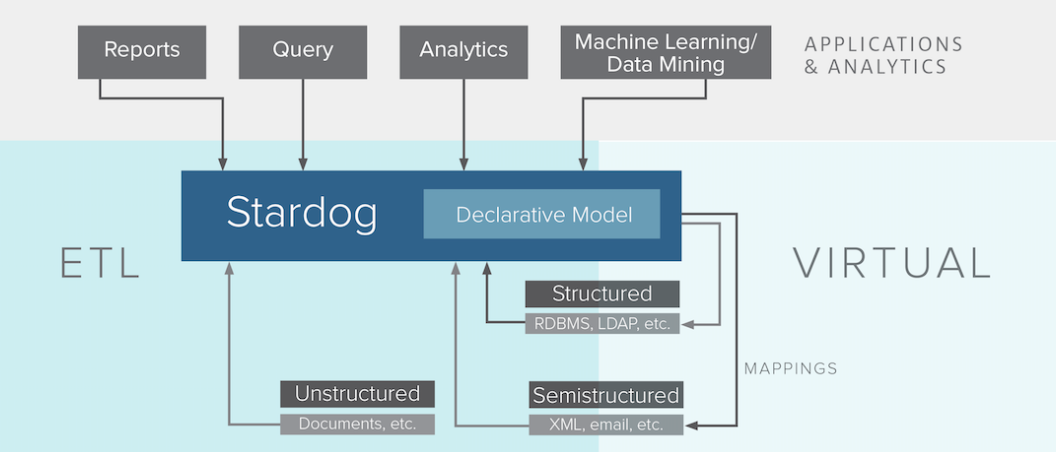
\includegraphics[width=\columnwidth]{../images/stardog-architecture.png}
  \caption{Architecture of Stardog Knowledge Graph Platform}\label{sa:archi}
\end{figure}
There are three broad components centered around the Stardog graph 
database within the Knowledge Graph Platform, namely ETL, Virtual and 
Applications and Analytics. Each component is designed to provide 
the services in a declarative way. 
\begin{itemize}
	\item ETL stands for Extract, Transform, and Load, which are three 
	database functions that are combined to extract data out of one database 
	and insert into another database. Figure~\ref{sa:archi} illustrates that 
	three main types of data: structured, semi-structured and unstructured 
	are extracted and incorporated into the core graph database: Stardog. 
	\item Virtual refers to the mapping of relational data into the RDF database 
	as named graphs but without materialization (as in the ETL 
	fashion)~\cite{hid-sp18-405-blog-stardog-virtual}. 
	\item Applications and Analytics include generating reports from the 
	database, querying the database and perform analysis using statistical 
	inference and probabilistic reasoning and also built-in 
	machine learning libraries such as Vowpal, Wabbit and 
	XGBoost~\cite{hid-sp18-405-blog-stardog-ml}~\cite{hid-sp18-405-blog-stardog-xgboost}.
\end{itemize}

\section{Key Features}
In this section, the author discusses several key features of Stardog 
including Virtual Graph, Integrity Constraints, OWL and Rule 
Reasoning, Stardog Studio, Machine Learning, 
High Availability Cluster, Integration with AWS and PCF etc.\

\subsection{Virtual Graph}
Virtual Graph is a feature that facilitates the mapping of relational data into 
the RDF databases. ``Stardog supports the standard W3C R2RML mapping 
language~\cite{hid-sp18-405-www-stardog-r2rml} for defining how data in a 
relational system maps to RDF graphs'' and ``the mapped triples 
representing the source relational data are considered to be in a named 
graph that is not present (i.e., not materialized) in the local RDF 
graph''~\cite{hid-sp18-405-blog-stardog-virtual}, hence, the named graph is 
considered virtual.

When dealing with unified data sources, users could either apply ETL 
(Extract, Transform, and Load) after materialization of the virtual graph or 
directly query the virtual graph using federated queries (virtual queries). 
Federated query performs a translation of a SPARQL query into a SQL query 
and the execution is through a relational database 
engine~\cite{hid-sp18-405-blog-stardog-virtual2}~\cite{hid-sp18-405-diego2017ontop-stardog}.
 Key trade-offs between these two operational models are summarized as 
 follows:
 \begin{itemize}
	\item Evaluation of queries over materialized data via ETL does not involve 
	any communication with the source system. This in general leads to better 
	query performance and independence of queries from the availability of 
	the source system~\cite{hid-sp18-405-blog-stardog-virtual}.
	\item Materialization, on the other hand, takes multiple steps and 
	resources for creating and storing tuples in RDF model, which is 
	time-consuming. Further, when the data points are modified frequently 
	before queried, materialization will lead to a worse performance compared 
	to virtual queries, which is essentially real-time reasoning.
\end{itemize}
Stardog offers both ways of unifying data, federated queries and 
materialization. The system allows users to switch between the two and the 
``choices can be made on a source by source 
basis''~\cite{hid-sp18-405-blog-stardog-virtual}.

\subsection{Integrity Constraints}
In Stardog, Integrity Constraints (IC) are used to validate RDF data based on 
constraints or rules imposed by the database users. Stardog supports 
multiple languages for specifying the rules including SPARQL and OWL, 
which allows querying and mapping these rules in SPARQL as 
well~\cite{hid-sp18-405-www-stardog-docs}. Implementation of such 
constraints allows the users to apply domain-specific knowledge to the data 
and align the knowledge with RDF.\@ Integrity Constraints can then be 
utilized in the reasoning procedure to ensure logical consistency and explain 
errors, which is the advantage of RDF database over plain property graph 
database in general. 

\subsection{OWL and Rule Reasoning}
Stardog’s OWL reasoning is based on the OWL 2 Direct Semantics Entailment 
Regime and Stardog performs reasoning at query time without inference 
materialization. In addition, Stardog provides explanation of an inference by 
``minimum set of statements explicitly stored in the database that, together 
with the schema and any valid inferences, logically justify the 
inference''~\cite{hid-sp18-405-www-stardog-docs}. Under the circumstances 
where OWL’s axiom-based approach is not adequate for the reasoning, 
Stardog allows User-defined rules as a complements and enhance the power 
of the reasoning by combining both OWL and rules into the system. 

\subsection{Stardog Studio}
Stardog Studio-the Knowledge Graph IDE, which is announced early 2018, is 
a front end developing tool for Stardog. It includes a SPARQL query 
notebook, which provides ``syntax highlighting, prefix auto-completion, and 
exporting results''~\cite{hid-sp18-405-blog-stardog-studio}. In addition, 
users could also ``execute SPARQL queries against Stardog database and 
view results inside Stardog studio and export query results to the file 
system''~\cite{hid-sp18-405-www-stardog-studio}.

Stardog Studio also provides the functionality of database management and 
security view. These allow the users to view and administer the Stardog 
databases as well as user, role and permissions for the Stardog 
system~\cite{hid-sp18-405-blog-stardog-studio}.

Additional features like visualization and cluster management tools are under 
development and expected in future 
releases~\cite{hid-sp18-405-www-stardog-studio}.

\subsection{Machine Learning}
With the built-in machine learning libraries such as Vowpal, Wabbit and 
XGBoost, Stardog could perform traditional machine learning with statistical 
inference and probabilistic 
models~\cite{hid-sp18-405-blog-stardog-xgboost}. 

Further, Machine Learning has been used in two unique ways supporting the 
knowledge graph. First, learning methods and algorithms are applied when 
creating  the Knowledge Graph which unifies different data sources. Second,  
machine learning is also utilized to obtain actionable insight from the data 
unified. For example, predictive analytics is used to predict nodes and
edges in a Knowledge Graph, and extract patterns from the data in order to 
make forecast based on those patterns~\cite{hid-sp18-405-blog-stardog-ml}.


\subsection{High Availability Cluster}
Stardog utilizes High Availability Clusters for uninterrupted operations, 
redundancy and high query volume~\cite{hid-sp18-405-www-stardog-docs}. 
The clusters aims at mitigating the risk of failure on a single machine by 
automatically creating multiple copies of the service with Apache ZooKeeper 
as the distributed coordination 
tool~\cite{hid-sp18-405-www-stardog-predictiveanalyticstoday}. The cluster 
size affects performance in two ways: larger cluster sizes perform better 
for reads and perform worse for writes compared to small cluster 
sizes~\cite{hid-sp18-405-www-stardog-docs}. 

\subsection{Integration with AWS and PCF}
The Stardog High Availability Cluster supports installation by Stardog 
Graviton, which complies to a single binary executable. This facilitates the 
integration with Amazon Web Services and users could easily deploy, 
configure, and launch a Stardog cluster on Amazon 
AWS~\cite{hid-sp18-405-blog-stardog-aws}. 

Besides, ``the integration with Pivotal enables applications running in Pivotal 
Cloud Foundry to natively connect to Stardog instances without having to 
manually wire apes to services''~\cite{hid-sp18-405-blog-stardog-pcf}. This 
has been made available by the announcement of Stardog Service Broker for 
Pivotal Cloud Foundry.

\section{Comparison with Related Technologies}
Stardog is a graph database with RDF as a primary data model. Besides 
Stardog, there are other leading RDF graph databases including 4Store, 
GraphDB and Sesame. On the contrary, there is another type of graph 
databases, often referred to as property graph, that applies general Graph 
DBMS model without RDF.\@ Neo4j is one of the leading technology in this 
category. In this section, Stardog will be compared to GraphDB and Neo4j, 
illustrating strengths and weaknesses of Stardog both within the category of 
RDF database and against the other category namely property graph 
database. A comparison of some of the system properties of the three graph 
databases are summarized in 
Table\ref{t:comparison}~\cite{hid-sp18-405-www-stardog-dbengines-neo4j}~\cite{hid-sp18-405-www-stardog-dbengines-graphdb}

\begin{table}[htb]
	\centering
	\caption{System Properties Comparison GraphDB vs.\ Neo4j vs.\ 
	Stardog}\label{t:comparison}
	\begin{tabular}{llll}
	Name & GraphDB & Neo4j & Stardog \\
		\toprule
	Database model&	Graph DBMS and RDF & Graph DBMS & Graph DBMS and 
	RDF \\
	\midrule
	DB-Engines Ranking (Graph DBMS) &\#12 &\#1 &\#10\\
	\midrule
	DB-Engines Ranking (RDF) &\#7 &N/A &\#6\\
	\midrule
	Developer & Ontotext &	Neo4j, Inc.	& Complexible Inc.\\
	\midrule
	Initial release	&2000 &	2007&	2010\\
	\midrule
	License &	commercial &	Open Source &	commercial \\
	\midrule
	Implementation language &	Java &	Java, Scala &	Java\\
	\midrule
	Any SQL supported &	SPARQL &	no	& SPARQL \\
	\midrule
	In-memory capabilities&no &no &			yes\\
	\midrule
	XML support&	no	& no& 	partially\\
	\bottomrule
	\end{tabular}
\end{table}

\subsection{Stardog vs.\ Neo4j}
Neo4j, as a leading property graph database (ranking \#1 by DB-Engines 
according to Table\ref{t:comparison}), has strength in the following aspects. 
First, it is highly flexible that most objects and relations could be represented 
as nodes and edges respectively in the graph. Second, it does not require 
schema or ontology and thus light-weighted compared to RDF databases. 
Finally, it has a relative simple graph structure for traversals and 
analysis~\cite{hid-sp18-405-robinson2013graphdatabase-stardog}. 

However, there are several important features of Stardog that property graph 
like Neo4j could not achieve. First, Neo4j only supports materialization of 
data. Virtualization of data (virtual graph) cannot be performed. Second, 
query language used by property languages such as Cypher and Gremlin lack 
the expressibility and ability to yield structured views of data compared to 
query languages like SPARQL~\cite{hid-sp18-405-angles2008expre-stardog}. 
Stardog uses SPARQL as a main query language and also supports all of 
Apache TinkerPop3 including 
Gremlin~\cite{hid-sp18-405-www-stardog-docs}. Finally, without RDF and 
OWL, property graph cannot impose integrity constraints, explanations, 
user-defined rules or reasoning, which are all achievable in 
Stardog~\cite{hid-sp18-405-www-stardog-dbengines-neo4j}~\cite{hid-sp18-405-www-stardog-docs}.
 
\subsection{Stardog vs.\ GraphDB}
Both Stardog and GraphDB support RDF models and share many important 
features including reasoning, user-defined rules, SPARQL query and machine 
learning modules. However, Stardog has the capability of Virtual Graph which 
avoids materialization when unifying data sources, which is a key strength 
compared to GraphDB.\@ GraphDB on the other hand, has a major advantage 
and focus on Natural Language Processing (NLP) and text mining by 
providing Ontotext Platform as an integrated text analysis 
system~\cite{hid-sp18-405-www-stardog-ontotext}, while Stardog only 
supports text analytics indirectly by providing connectors to other NLP 
libraries OpenNLP~\cite{hid-sp18-405-www-stardog-docs}. 

Besides capabilities, researchers have been testing and comparing the 
performance of RDF graphs including GraphDB and Stardog. Based on 
experiments on real data, Ledvinka, Martin and K{\v{r}}emen concluded that 
``GraphDB, (and storages performing materialization in general) has a major 
disadvantage in that the user has to specify inference level before actually 
inserting data into the storages. Real time reasoning (like Stardog), on the 
other hand, lets the user choose reasoning level at the query time. However, 
GraphDB appears to be more suitable for the object-oriented application 
access scenario, in which frequent data updates are 
expected''~\cite{hid-sp18-405-ledvinka2015object-stardog}. In a more recent 
study, Luyen and his colleagues compared six RDF data models: 4Store, 
Virtuoso, Stardog, GraphDB, Sesame and Jena Fuseki (TDB) using large RDF 
graphs. They found that Stardog gives the best results compared to the 
criteria: Data Loading, Data Search and Data Inference therefore they stated 
that in general outperforms the other five candidates for their 
Benchmark~\cite{hid-sp18-405-luyen2016development-stardog}.


\section{License}
As a commercial software, Stardog is priced for community, developer and 
enterprise tiers. The community version is free with 10 databases, 25 million 
triples 
per database and the developer version offers a free 30-day trial with 
unlimited data or 
machines~\cite{hid-sp18-405-www-stardog-predictiveanalyticstoday}. The 
enterprise version comes with a server management module and customer 
support by both phone and email~\cite{hid-sp18-405-www-stardog-docs}.


\section{Conclusion}
Stardog, as a commercial RDF-based graph database, supports data 
unification using both materialization and virtualization methods, and allows 
semantic reasoning and logical inferences by utilizing integrity constraints, 
OWL, and user-defined rules. The advantages of virtual graph, SPARQL 
query, and reasoning capability has made it an alternative to property graph 
databases, such as Neo4j. 


\begin{acks}

  The author would like to thank Dr.~Gregor~von~Laszewski for his
  support and suggestions to write this paper.

\end{acks}

\bibliographystyle{ACM-Reference-Format}
\bibliography{report} 

